%%%%%%%%%%%%%%%%%%%%%%%%%%%%%%%%%%%%%%%%%%
% Revised Introduction Section
%%%%%%%%%%%%%%%%%%%%%%%%%%%%%%%%%%%%%%%%%%
We start in \Cref{AboutVFT} with providing a brief overview of the company, Vermiculus Financial Technology, and its activities. \Cref{Background} presents background information on the topic of clearing and the need for dependency modeling. \Cref{LiteratureReview} offers a brief overview of the literature and history of copulas. \Cref{Purpose} outlines the purpose, intended contributions, and research questions of this project. Finally, \Cref{Limitations} describes the limitations of this project.

\subsection{About Vermiculus Financial Technology} \label{AboutVFT}
Vermiculus Financial Technology is a software company that develops systems for financial transactions. Its three main areas of operation are trading systems, clearing systems, and \gls{CSD} systems. Trading systems match buy and sell orders in the market and determine the price at which trades are executed. Clearing systems reduce counterparty risk in financial transactions by serving as a central hub through which all transactions flow. \gls{CSD} systems track the ownership of every stock on an exchange. This project relates to the clearing segment of Vermiculus’s activities.

\subsection{Background}\label{Background}
Clearing systems exist to minimize counterparty risk in financial transactions\footnote{See "Systems in the financial infrastructure", \textit{Sveriges Riksbank}, Updated: 2024-06-28, \url{https://www.riksbank.se/en-gb/financial-stability/the-financial-system/the-financial-infrastructure/systems-in-the-financial-infrastructure/}, Last Accessed: 2025-01-29.}. Counterparty risk refers to the possibility that one party in a transaction will not fulfill its obligations, effectively defaulting on the agreement\footnote{See "Counterparty Risk", \textit{Office of the Comptroller of the Currency}, \url{https://www.occ.treas.gov/topics/supervision-and-examination/capital-markets/financial-markets/counterparty-risk/index-counterparty-risk.html}, Last Accessed: 2025-01-29.}.


A clearing house acts as an intermediary in all transactions, selling to all buyers and buying from all sellers\footnote{See Akhilesh Ganti, "Clearinghouse: An Essential Intermediary in the Financial Markets", \textit{Investopedia}, Updated: 2023-02-07, \url{https://www.investopedia.com/terms/c/clearinghouse.asp}. Last Accessed: 2025-01-27.}. Consequently, each party faces only the clearing house as its counterparty, effectively removing counterparty risk. This is illustrated in \Cref{fig:CCP} by AnalystPrep\footnote{See "Central Clearing - Financial markets and products part 1", \textit{Analyst Prep}. Updated: 2023-08-02, \url{https://analystprep.com/study-notes/frm/part-1/financial-markets-and-products/central-clearing/}, Last Accessed: 2025-01-29.}, where the right panel shows that the clearing members, marked B (usually banks), interact only with the clearing house (marked CCP). In this arrangement, as long as the clearing house remains solvent, trades can proceed even if a clearing member defaults. However, the clearing house does not provide this service for free; each party must post collateral to cover potential losses in the event of a member default. The clearing house earns revenue through fees and transaction costs, making the model viable.

In contrast, without central clearing, market participants trade directly with each other. In such a bilateral setup, both parties are exposed to counterparty risk from the time the trade is made until it is settled. For instance, the buyer might lack the funds to pay, or the seller might not possess the agreed asset. This is illustrated in the left panel of Figure~\ref{fig:CCP}, where clearing members (marked B) face each other in trades. If one member defaults, the counterparties may not receive payment, potentially triggering a chain reaction of defaults—an effect known as contagion.





\begin{figure}[ht]
    \centering
    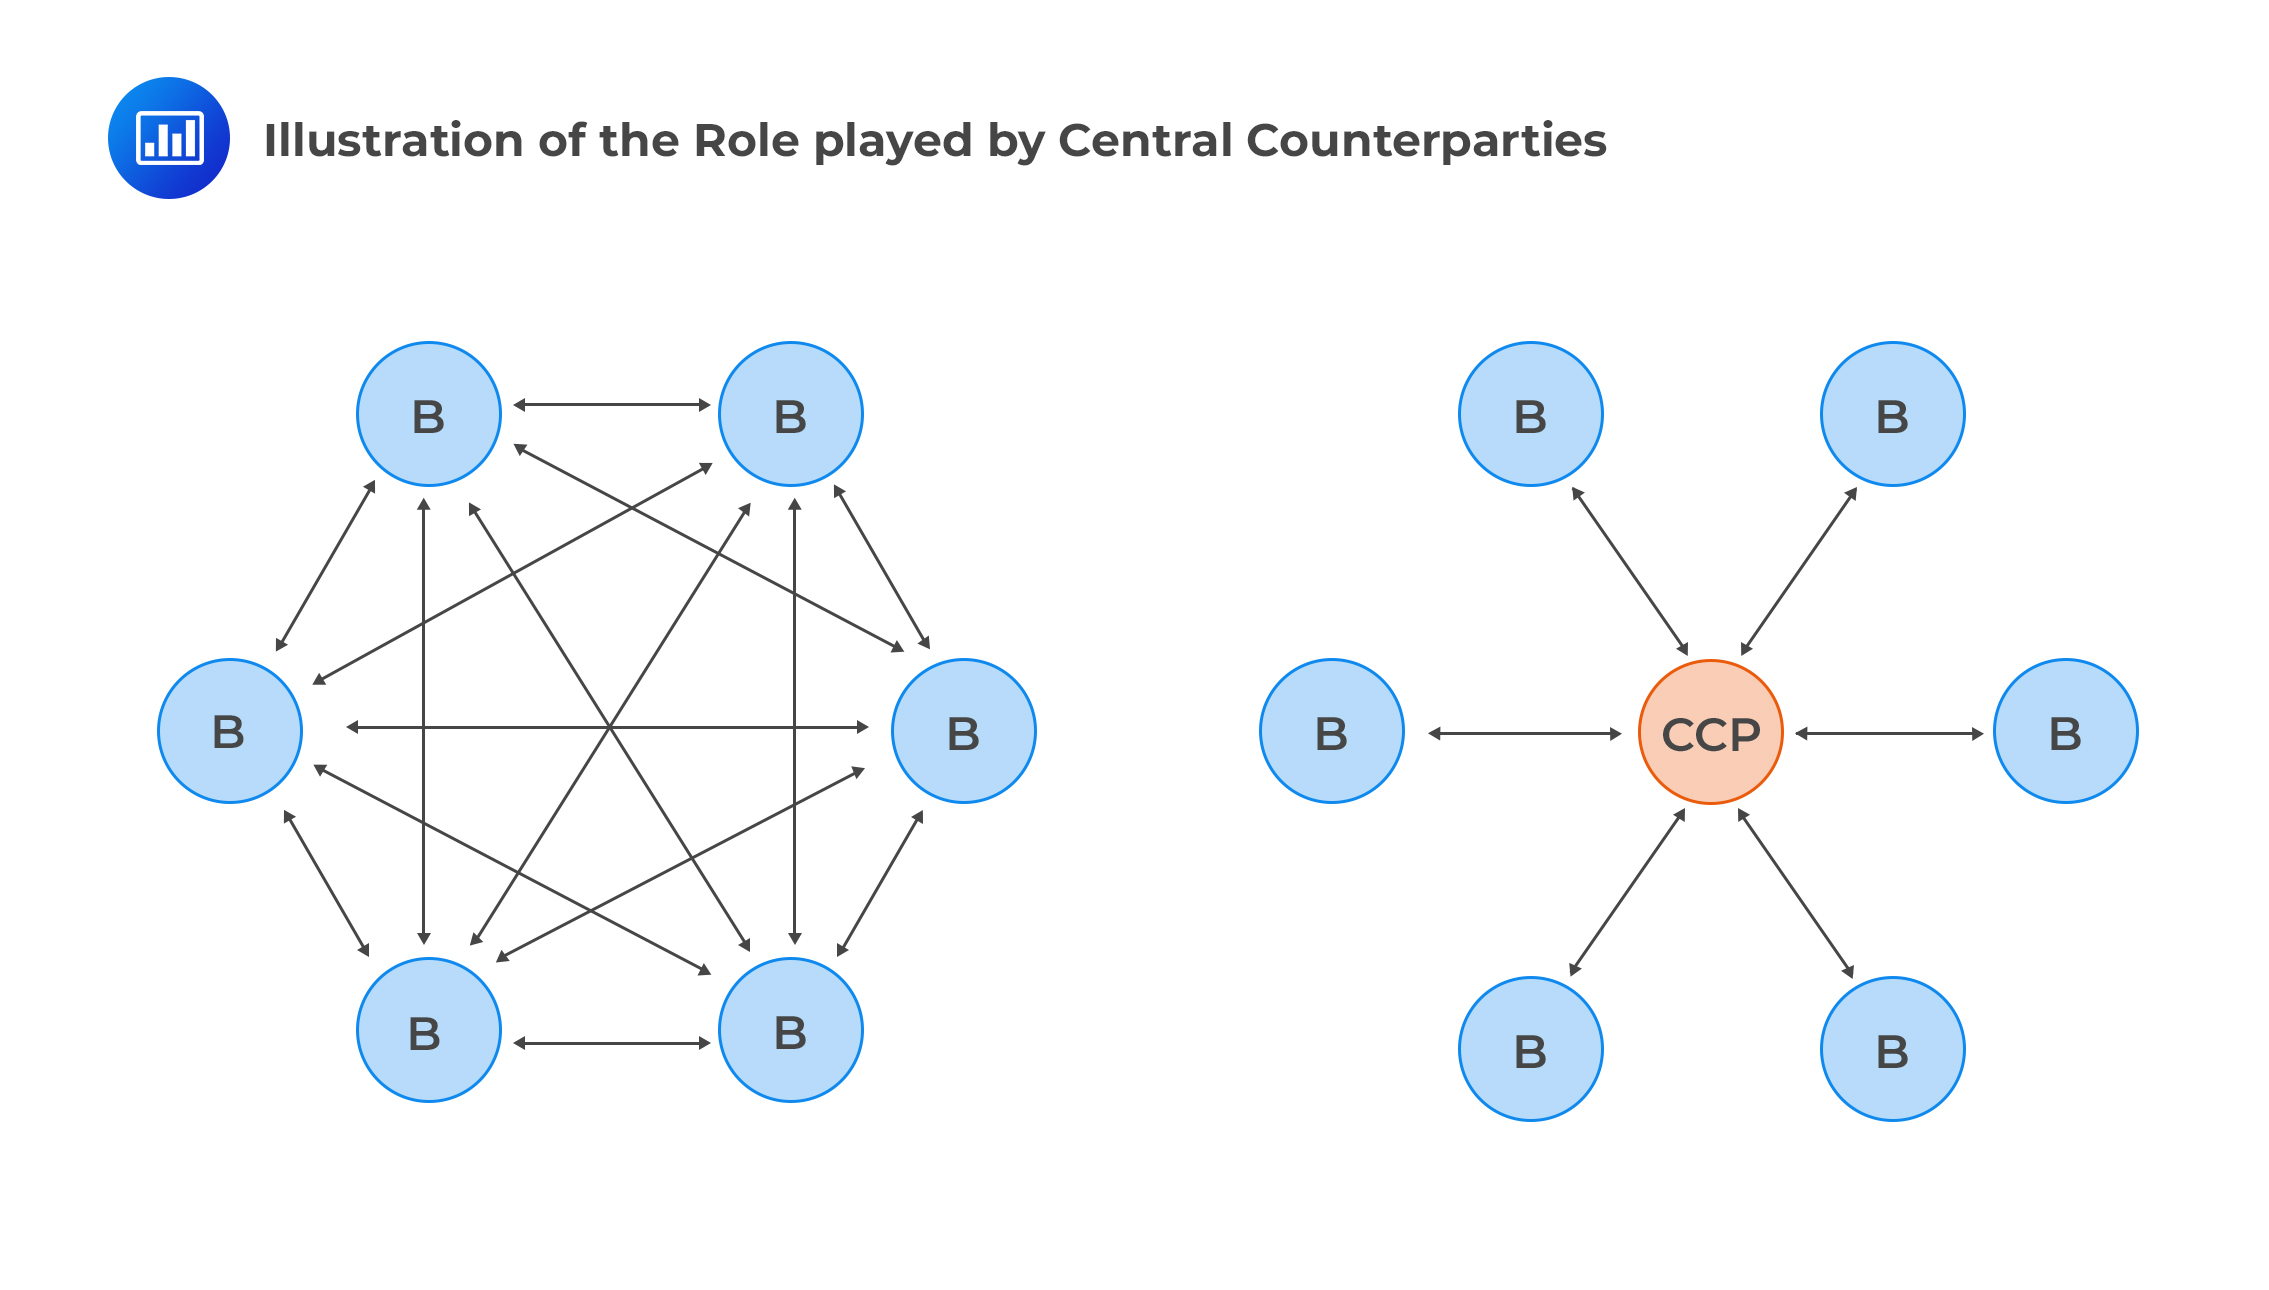
\includegraphics[width=0.7\linewidth]{1Introduction/pictures/CCPvisual .jpg}
    \caption{Bilateral and central counterparty clearing compared. The left image depicts bilateral clearing, while the right image shows central counterparty clearing. Illustration sourced from AnalystPrep\protect\footnotemark[\value{footnote}].}
    \label{fig:CCP}
\end{figure}

To determine the required collateral, the risk associated with each clearing member's portfolio must be assessed. Historically, this was done using the \gls{SPAN} framework, developed by the Chicago Mercantile Exchange\footnote{See "CME SPAN Methodology Overview", \textit{CME Group}, \url{https://www.cmegroup.com/solutions/risk-management/performance-bonds-margins/span-methodology-overview.html\#how-it-works}. Last Accessed: 2025-01-29.}. \gls{SPAN} defines various scenarios based on changes in price, volatility, and time to maturity for derivatives, and calculates the resulting changes in security values.

Following the 2008 global financial crisis, greater emphasis was placed on risk management. More recently, a shift toward using \gls{VaR} has occurred\footnote{See Rafik Mrabet, "Navigating a New Era in Derivatives Clearing", \textit{FIA}, Updated: 2024-01-04, \url{https://www.fia.org/marketvoice/articles/navigating-new-era-derivatives-clearing}. Last Accessed: 2025-01-26.}. \gls{VaR} is defined as the maximum expected portfolio loss over a specified time horizon at a given confidence level\footnote{See "Value-at-risk (VAR)", \textit{Risk.net}, \url{https://www.risk.net/definition/value-at-risk-var}. Last Accessed: 2025-01-29.}. Several methods exist for calculating \gls{VaR}, including historical, parametric, and \gls{MC} simulation approaches\footnote{See "Value-at-risk (VAR)", \textit{Corporate Finance Institute}, \url{https://corporatefinanceinstitute.com/resources/career-map/sell-side/risk-management/value-at-risk-var/}. Last Accessed: 2025-01-29.}.  

Historical \gls{VaR} uses past asset returns to compute portfolio returns at each time point. These returns are then ordered, and the \gls{VaR} is determined by selecting the percentile corresponding to the confidence level. This method realistically captures asset dependence as it is based on observed market data\footnotemark[\value{footnote}]. However, it may be inadequate due to the limited availability of extreme observations—particularly relevant for \gls{VaR}, which focuses on tail risk.

Parametric \gls{VaR} assumes that asset returns follow a known distribution. In simpler cases, the Gaussian distribution is used, with the mean vector and covariance matrix estimated from the data. This distribution is then employed to calculate the \gls{VaR} such that the probability of loss exceeding it matches the confidence level\footnotemark[\value{footnote}]. The advantage of this method lies in its simplicity and ease of use. However, it requires that the returns follow the assumed distribution, which may not always be realistic.

\gls{MC} \gls{VaR} generates artificial return scenarios by simulating random numbers from specified distributions\footnotemark[\value{footnote}]. This method is highly flexible and particularly well-suited for calculating risks associated with various types of financial instruments by simulating plausible scenarios for the portfolio’s underlying assets.

To compute \gls{MC} \gls{VaR}, the simulated returns must capture the dependence structure between assets. This can be done using covariance matrices or copulas. There are various types of copulas available, providing many modeling options—especially when fitting marginal distributions separately. This naturally leads to the purpose of this project, which follows a brief review of the literature and history of copulas.

\subsection{Literature Review and History}\label{LiteratureReview}
\Citet[pp.~1–3]{DuranteSempi2010} provide an overview of the history of copulas, which is briefly summarized here. The origins of copula theory can be traced back to Fréchet’s 1951 work on functions linking marginal and joint distributions. In 1959, Sklar introduced the term "copula" in his work on statistical metric spaces, culminating in Sklar’s theorem—a cornerstone of copula theory. About 15 years later, Schweizer began using copulas to construct dependence measures, and in 1983, Sklar and Schweizer co-authored a book on copulas. The late 1990s saw the publication of two influential books—one by Nelsen and one by Joe—which helped boost interest in copulas. As noted by Embrechts, their use in finance, particularly in models moving away from i.i.d. assumptions, contributed significantly to their rising popularity.

Despite their versatility, copulas can be difficult to apply in high-dimensional settings. In 2022, \Citet{ZengWang2022} introduced the \gls{NC}, a novel method for modeling dependence by approximating copula functions using \gls{NN}s. This approach serves as the starting point for this project.

\subsection{Purpose}\label{Purpose}
In this project we investigate various copula-based methods for modeling dependence and to clarify which methods are most appropriate for different types of data. The contributions in this thesis is to enhance understanding of how these methods can be applied in practice. In particular, the focus is on utilizing the \gls{NC} to model the dependence between log returns of different assets. To increase its practical applicability in risk management, this project explores an alternative approach to fitting marginal distributions within the \gls{NC} framework and develops a method for sampling from the \gls{NC}. 

Furthermore, the study examines which copula methods are best suited to various dependence structures and evaluates whether the \gls{NC} consistently outperforms traditional methods. Comparisons will be made between the \gls{NC} and other copulas, and strategies for training the \gls{NC} to produce reliable results will be explored. Since the \gls{NC} is a relatively new method with limited practical deployment, understanding its capabilities and limitations is essential.

The research questions guiding this project are as follows:
\begin{compactenum}[{\bfseries RQ}1]
    \item \label{item:RQ1} Is the marginal distribution used in the \gls{NC} adequate?
    \item \label{item:RQ2} How should the neural copula function be trained to yield consistently reliable results?
    \item \label{item:RQ3} Can a neural copula more accurately model the dependence between asset returns than other copula methods?
\end{compactenum}
\newcommand{\RQone}{{\bfseries RQ}\ref{item:RQ1} }
\newcommand{\RQtwo}{{\bfseries RQ}\ref{item:RQ2} }
\newcommand{\RQthree}{{\bfseries RQ}\ref{item:RQ3} }

\subsection{Limitations}\label{Limitations}
To define the scope of this project, several limitations were established during its initial phase:

\begin{compactenum}
    \item A selected subset of traditional copulas was chosen for comparison with the \gls{NC}.
    \item The portfolios analyzed will be limited to two assets to enhance interpretability and enable visualization.
    \item Artificially simulated data will be used to control the dependence between assets and to ensure consistent evaluation across methods. This also allows control over the marginal distributions, focusing the evaluation solely on the copula methods.
    \item The main emphasis of this report is the implementation and evaluation of the \gls{NC}. Once this is accomplished, additional performance measures will be considered.
\end{compactenum}

Additional limitations were introduced during the project to maintain feasibility, such as restricting the number of datasets and hyperparameters tested.

This thesis is structured as follows: \Cref{sec:theory} introduces the theoretical background necessary to understand the methods used. \Cref{sec:Method} outlines the methodology. \Cref{sec:Results} presents and discusses the results of the conducted tests. Finally, \Cref{sec:Conclusion} summarizes the findings and suggests avenues for future research.




% %%%%%%%%%%%%%%%%%%%%%%%%%%%%%%%%%%%%%%%%%%
% % Old from before fixing using chatgpt
% %%%%%%%%%%%%%%%%%%%%%%%%%%%%%%%%%%%%%%%%%%
% This section introduces the project and its purpose. \Cref{AboutVFT} will give a brief overview of the company, Vermiculus Financial Technology, and its activities. \Cref{Background} will give a background to the topic of clearing and the need for dependency modeling. \Cref{LiteratureReview} will give a brief overview of the literature  and history of copulas. \Cref{Purpose} will present the purpose, intended contributions, and research questions of this project. Finally, \Cref{Limitations} will present the limitations of this project. Finally, \Cref{Limitations} will present the limitations of this project.

% \subsection{About Vermiculus Financial Technology} \label{AboutVFT}
% Vermiculus Financial Technology is a software company that builds systems for financial transactions. Its three main areas of operations are trading systems, clearing systems, and \gls{CSD} systems. Trading systems match buy and sell orders in the market and find the price at which trades should be executed. Clearing systems reduce counterparty risk in financial transactions by acting as the central hub through which all transactions flow. \gls{CSD} systems keep track of who owns every stock on an exchange. This project will be related to the clearing section of Vermiculus activities. 

% \subsection{Background}\label{Background}
% Clearing systems are in place to minimize counterparty risk in financial transactions\footnote{See \url{https://www.riksbank.se/en-gb/financial-stability/the-financial-system/the-financial-infrastructure/systems-in-the-financial-infrastructure/}. Last Accessed: 2025-01-29}. Counterparty risk is the risk of having the other party in a transaction not fulfilling its end of a deal and hence defaulting on its obligations\footnote{See \url{https://www.occ.treas.gov/topics/supervision-and-examination/capital-markets/financial-markets/counterparty-risk/index-counterparty-risk.html}. Last Accessed: 2025-01-29}. 
% The clearing house acts as a middleman in all transactions, selling to all buyers and buying from all sellers\footnote{See \url{https://www.investopedia.com/terms/c/clearinghouse.asp}. Last Accessed: 2025-01-27}. Hence, each party only faces the clearing house as their counterparty, removing the counterparty risk, this has been nicely illustrated\footnote{See \url{https://analystprep.com/study-notes/frm/part-1/financial-markets-and-products/central-clearing/}. Last Accessed: 2025-01-29}. In the right part of Figure~\ref{fig:CCP} we can see the clearing members marked B, usually banks, that only face the clearing house marked CCP. In this system, as long as the clearing house does not go bankrupt, trades can go through even if a clearing member defaults on their commitment. The clearing house does not offer this risk removal for free; rather, it requires each party to post collateral covering the costs if a clearing member defaults. The clearinghouse makes money from fees and transaction costs, making it worthwhile.

% The alternative to centrally cleared trading is that each market participant trades directly with each other. In this case, both sides of a transaction are exposed to counterparty risk from when making a trade until it has been settled. The risk in this scenario is that the buyer does not have enough money to pay or that the seller does not have the asset it has agreed to sell. This is nicely illustrated\footnotemark[\value{footnote}] in the left part of Figure \ref{fig:CCP}. We can see that each clearing member, marked B, faces each other if having the buy and sell side of the same position. In this system, if one of the clearing members defaults, it can impact the other clearing members, who will not get their money. This can cause contagion, so if one clearing member goes bankrupt, others may follow suit. 

% \begin{figure}[ht]
%     \centering
%     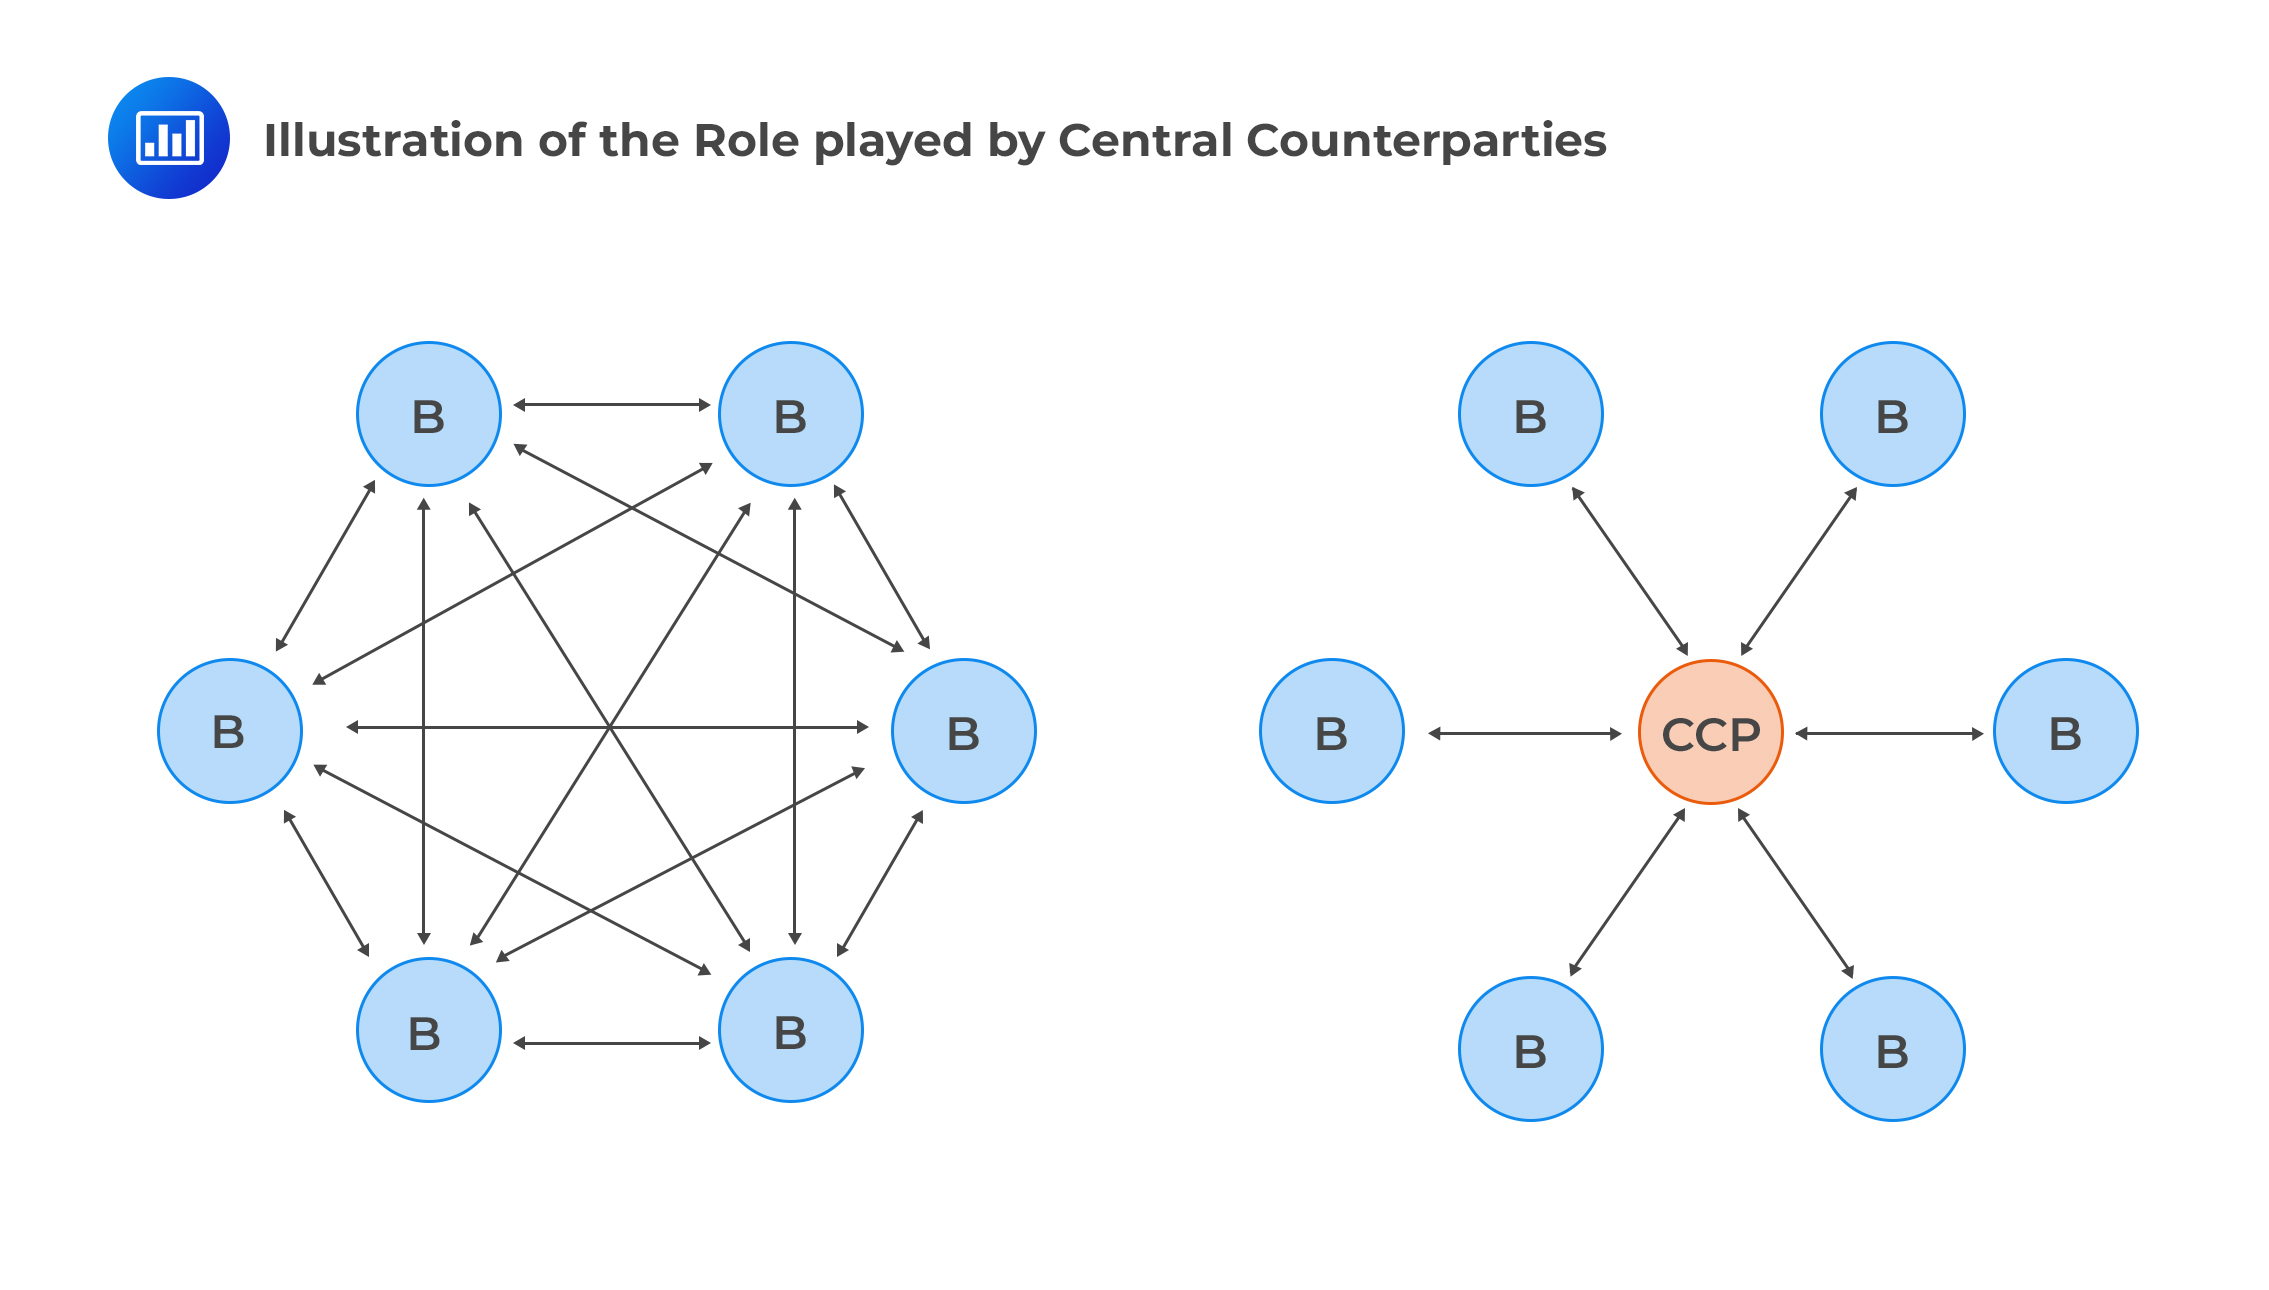
\includegraphics[width=0.7\linewidth]{1Introduction/pictures/CCPvisual .jpg}
%     \caption{Bilateral and central counterparty clearing compared. The left picture shows a system of parties that are clearing transactions bilaterally. The right picture shows a system where central counterparty clearing is used. This illustration was found at AnalystPrep\protect\footnotemark[\value{footnote}]. }
%     \label{fig:CCP}
% \end{figure}

% To determine how much collateral is required from each clearing member, the risk of its portfolio must be measured. Historically this has been done using a framework called \gls{SPAN} that was developed by Chicago Mercantile Exchange\footnote{See \url{https://www.cmegroup.com/solutions/risk-management/performance-bonds-margins/span-methodology-overview.html\#how-it-works}.  Last Accessed: 2025-01-29}. The \gls{SPAN} framework has several scenarios based on changes in price, volatility, and time to maturity for derivatives. These scenarios are then used to calculate what change in value they would have for some security. Since the global financial crisis in 2008, more focus has been put on risk management. In later years a shift towards using \gls{VaR} has taken place\footnote{See \url{https://www.fia.org/marketvoice/articles/navigating-new-era-derivatives-clearing}. Last Accessed: 2025-01-26}. \gls{VaR} is a measure defined as the maximum expected loss in portfolio value over a time horizon for some level of confidence\footnote{See \url{https://www.risk.net/definition/value-at-risk-var}. Last Accessed: 2025-01-29}. There are several ways of calculating value at risk \gls{VaR} such as historical, parametric, and \gls{MC} simulated among others \footnote{See \url{https://corporatefinanceinstitute.com/resources/career-map/sell-side/risk-management/value-at-risk-var/}. Last Accessed: 2025-01-29}.  

% Historical \gls{VaR} uses historical returns from the different assets in it to calculate the return of the portfolio at each time step. These portfolio returns are then ordered and the percentile corresponding to the confidence level is calculated giving the \gls{VaR}. This method has advantages and disadvantages. The advantage is that the dependence between assets is completely realistic as it comes from the true observations on the market\footnotemark[\value{footnote}]. A disadvantage is however that this model can be insufficient because the observations from the data are limited. This might sound strange but when observations falling in the tails of a distribution is of course rare. This means that for \gls{VaR}, which focuses on the lower tail, the amount of data available might not be enough to precisely determine the \gls{VaR}.  

% Parametric \gls{VaR} assumes that the returns for an asset are generated from some distribution. These returns are then used for calculating the described characteristics of the distribution. In simple \gls{VaR} models, the Gaussian distribution is often used, in which case the mean vector and covariance matrix are estimated. This distribution is then used to calculate the \gls{VaR} so that the probability of ending up below the limit aligns with the confidence\footnotemark[\value{footnote}]. This method has the advantage that it is easy to use and understand. It has a disadvantage in that it requires the data to follow some known distribution which might not always be a realistic assumption.  

% \gls{MC} \gls{VaR} utilizes simulated random numbers to generate artificial return scenarios from which the \gls{VaR} can be calculated\footnotemark[\value{footnote}]. \gls{MC} simulations have a major advantage over the other methods mentioned in that they can be used for calculating the risks of different types of financial instruments. This is done by simulating plausible scenarios for the underlying assets of a portfolio.  

% The returns used for computing \gls{MC} \gls{VaR} need to be simulated from distributions with dependence that reflect how different assets move in relation to one another. Several methods can be used to do this, such as using covariance matrices or copulas. There are several different types of copulas to use, meaning that there are many alternative methods to choose from, especially when also having the task of fitting marginal distributions to the data. This leads us to the purpose of this project, but first, a brief overview of the literature and history of copulas will be given.

% \subsection{Literature review and history}\label{LiteratureReview}
% \Citet[pp.~1-3]{DuranteSempi2010} provides an overview of the history of copulas. In this paragraph, a brief summary of their overview will be given. It is possible to mark the starting point of the copula theory to the work of Fréchet in 1951, studying the class of functions linking marginal distributions to joint distributions. In 1959 Sklar introduced the term copula in his work on statistical metric spaces. This resulted in Sklar's theorem which is central to the theory of copulas. Roughly 15 years later Schweizer introduced the use of copulas to construct dependence measures. In 1983 Sklar and Schweizer published  a book on copulas. During the late 1990s two books on copulas were published, one by Nelsen and one by Joe. The interest in copulas increased significantly due to applications in finance as said by Embrechts. Particularly, the move from models using i.i.d. assumptions was contributing to the increased interest in copulas. 

% A challenge with copulas is that they are not always easy to use, particularly when the dimensionality of the data increases. In 2022 \Citet{ZengWang2022} introduced the \gls{NC} which is a new method of modeling dependence by approximating a copula function using \gls{NN}s. This method will be the starting point of this project. 


% % Copulas are widely used in mathematical finance \Citet[p.~1]{Umberto2004copulaMethods}. The use cases are many but some of the most common are pricing of basket options \Citet[pp.~279-280]{Umberto2004copulaMethods}, \gls{VaR} \Citet[p.~253]{Alexander2008} calculations, and credit risk \Citet[p.~1]{Umberto2004copulaMethods}. It is particularly useful because it allows for modeling dependence separate from the marginal distributions which is useful when returns are not both normally or students $t$ distributed \Citet[p.~253]{Alexander2008}. 
% % \todo{Reference to the summary article on copulas. Remove the connection to mathematical finance.}


 
% \subsection{Purpose}\label{Purpose}
% The purpose of this project is to investigate different copula methods of modeling dependence and to provide clarity about which method to use for what type of data. The intended contribution of this project is to provide a better understanding of how different methods of modeling dependence can be used in practice. More specifically, the focus will be on how to use the \gls{NC} to model dependence between log returns of different assets. To make the \gls{NC} method more useful in practical risk applications, an alternative method for fitting the \gls{NC} marginal distributions will be investigated. Additionally, an approach for sampling the \gls{NC} will be developed to make it useful in practice. Finally, we will investigate what copula method to use when and investigate if the \gls{NC} outperforms other methods for all types of dependence structures. This will be done by comparing the \gls{NC} to other copula methods and by investigating how the \gls{NC} can be trained to obtain reliable results. The \gls{NC} is a new method that has not been widely used in practice yet, so it is important to understand how it can be used and what its limitations are. 

% The research questions that will be studied in this project are introduced below:
% %\paragraph*{Research questions.}
% \begin{compactenum}[{\bfseries RQ}1]
%     \item \label{item:RQ1} Is the marginal distribution used in the \gls{NC} adequate to use?
%     \item \label{item:RQ2} How should the neural copula function be trained to obtain consistently reliable results?
%     \item \label{item:RQ3} Can a neural copula be used to better model the dependence between asset returns than other copulas?
% \end{compactenum}
% \newcommand{\RQone}{{\bfseries RQ}\ref{item:RQ1} }
% \newcommand{\RQtwo}{{\bfseries RQ}\ref{item:RQ2} }
% \newcommand{\RQthree}{{\bfseries RQ}\ref{item:RQ3} }

% \subsection{Limitations}\label{Limitations}
% To restrict the scope of this project some limitations was determined during the initial phase of the project.

% \begin{compactenum}
%     \item A selection of traditional copulas to compare the \gls{NC} to was made. 
%     \item The number of assets in the portfolios will be limited to two assets. This will help with interpretability as it allows for visualization. 
%     \item The data used will be artificially simulated to control the dependence between the assets in the portfolios and to be able to evaluate each method under consistent conditions. This also allows us to control the marginal distributions of the data, making the test only focus on the copula methods.  
%     \item The main focus of this report is to implement and evaluate the \gls{NC}. When this is done, other measures will be considered. 
% \end{compactenum}
% Additional limitations have been made along the way to make the project more manageable. For example, the number of datasets tested, and the number of hyper parameters tested.  

% This thesis is structured as follows: \Cref{sec:theory} will give an introduction to the theory, necessary for understanding the methods used in this project. \Cref{sec:Method} will present the methods used in this project. \Cref{sec:Results} will present and discuss the results of the tests conducted. Finally, \Cref{sec:Conclusion} will summarize the findings and suggest future work. 


